% Options for packages loaded elsewhere
\PassOptionsToPackage{unicode}{hyperref}
\PassOptionsToPackage{hyphens}{url}
\PassOptionsToPackage{dvipsnames,svgnames,x11names}{xcolor}
%
\documentclass[
  letterpaper,
  DIV=11,
  numbers=noendperiod]{scrartcl}

\usepackage{amsmath,amssymb}
\usepackage{iftex}
\ifPDFTeX
  \usepackage[T1]{fontenc}
  \usepackage[utf8]{inputenc}
  \usepackage{textcomp} % provide euro and other symbols
\else % if luatex or xetex
  \usepackage{unicode-math}
  \defaultfontfeatures{Scale=MatchLowercase}
  \defaultfontfeatures[\rmfamily]{Ligatures=TeX,Scale=1}
\fi
\usepackage{lmodern}
\ifPDFTeX\else  
    % xetex/luatex font selection
\fi
% Use upquote if available, for straight quotes in verbatim environments
\IfFileExists{upquote.sty}{\usepackage{upquote}}{}
\IfFileExists{microtype.sty}{% use microtype if available
  \usepackage[]{microtype}
  \UseMicrotypeSet[protrusion]{basicmath} % disable protrusion for tt fonts
}{}
\makeatletter
\@ifundefined{KOMAClassName}{% if non-KOMA class
  \IfFileExists{parskip.sty}{%
    \usepackage{parskip}
  }{% else
    \setlength{\parindent}{0pt}
    \setlength{\parskip}{6pt plus 2pt minus 1pt}}
}{% if KOMA class
  \KOMAoptions{parskip=half}}
\makeatother
\usepackage{xcolor}
\setlength{\emergencystretch}{3em} % prevent overfull lines
\setcounter{secnumdepth}{5}
% Make \paragraph and \subparagraph free-standing
\makeatletter
\ifx\paragraph\undefined\else
  \let\oldparagraph\paragraph
  \renewcommand{\paragraph}{
    \@ifstar
      \xxxParagraphStar
      \xxxParagraphNoStar
  }
  \newcommand{\xxxParagraphStar}[1]{\oldparagraph*{#1}\mbox{}}
  \newcommand{\xxxParagraphNoStar}[1]{\oldparagraph{#1}\mbox{}}
\fi
\ifx\subparagraph\undefined\else
  \let\oldsubparagraph\subparagraph
  \renewcommand{\subparagraph}{
    \@ifstar
      \xxxSubParagraphStar
      \xxxSubParagraphNoStar
  }
  \newcommand{\xxxSubParagraphStar}[1]{\oldsubparagraph*{#1}\mbox{}}
  \newcommand{\xxxSubParagraphNoStar}[1]{\oldsubparagraph{#1}\mbox{}}
\fi
\makeatother

\usepackage{color}
\usepackage{fancyvrb}
\newcommand{\VerbBar}{|}
\newcommand{\VERB}{\Verb[commandchars=\\\{\}]}
\DefineVerbatimEnvironment{Highlighting}{Verbatim}{commandchars=\\\{\}}
% Add ',fontsize=\small' for more characters per line
\usepackage{framed}
\definecolor{shadecolor}{RGB}{241,243,245}
\newenvironment{Shaded}{\begin{snugshade}}{\end{snugshade}}
\newcommand{\AlertTok}[1]{\textcolor[rgb]{0.68,0.00,0.00}{#1}}
\newcommand{\AnnotationTok}[1]{\textcolor[rgb]{0.37,0.37,0.37}{#1}}
\newcommand{\AttributeTok}[1]{\textcolor[rgb]{0.40,0.45,0.13}{#1}}
\newcommand{\BaseNTok}[1]{\textcolor[rgb]{0.68,0.00,0.00}{#1}}
\newcommand{\BuiltInTok}[1]{\textcolor[rgb]{0.00,0.23,0.31}{#1}}
\newcommand{\CharTok}[1]{\textcolor[rgb]{0.13,0.47,0.30}{#1}}
\newcommand{\CommentTok}[1]{\textcolor[rgb]{0.37,0.37,0.37}{#1}}
\newcommand{\CommentVarTok}[1]{\textcolor[rgb]{0.37,0.37,0.37}{\textit{#1}}}
\newcommand{\ConstantTok}[1]{\textcolor[rgb]{0.56,0.35,0.01}{#1}}
\newcommand{\ControlFlowTok}[1]{\textcolor[rgb]{0.00,0.23,0.31}{\textbf{#1}}}
\newcommand{\DataTypeTok}[1]{\textcolor[rgb]{0.68,0.00,0.00}{#1}}
\newcommand{\DecValTok}[1]{\textcolor[rgb]{0.68,0.00,0.00}{#1}}
\newcommand{\DocumentationTok}[1]{\textcolor[rgb]{0.37,0.37,0.37}{\textit{#1}}}
\newcommand{\ErrorTok}[1]{\textcolor[rgb]{0.68,0.00,0.00}{#1}}
\newcommand{\ExtensionTok}[1]{\textcolor[rgb]{0.00,0.23,0.31}{#1}}
\newcommand{\FloatTok}[1]{\textcolor[rgb]{0.68,0.00,0.00}{#1}}
\newcommand{\FunctionTok}[1]{\textcolor[rgb]{0.28,0.35,0.67}{#1}}
\newcommand{\ImportTok}[1]{\textcolor[rgb]{0.00,0.46,0.62}{#1}}
\newcommand{\InformationTok}[1]{\textcolor[rgb]{0.37,0.37,0.37}{#1}}
\newcommand{\KeywordTok}[1]{\textcolor[rgb]{0.00,0.23,0.31}{\textbf{#1}}}
\newcommand{\NormalTok}[1]{\textcolor[rgb]{0.00,0.23,0.31}{#1}}
\newcommand{\OperatorTok}[1]{\textcolor[rgb]{0.37,0.37,0.37}{#1}}
\newcommand{\OtherTok}[1]{\textcolor[rgb]{0.00,0.23,0.31}{#1}}
\newcommand{\PreprocessorTok}[1]{\textcolor[rgb]{0.68,0.00,0.00}{#1}}
\newcommand{\RegionMarkerTok}[1]{\textcolor[rgb]{0.00,0.23,0.31}{#1}}
\newcommand{\SpecialCharTok}[1]{\textcolor[rgb]{0.37,0.37,0.37}{#1}}
\newcommand{\SpecialStringTok}[1]{\textcolor[rgb]{0.13,0.47,0.30}{#1}}
\newcommand{\StringTok}[1]{\textcolor[rgb]{0.13,0.47,0.30}{#1}}
\newcommand{\VariableTok}[1]{\textcolor[rgb]{0.07,0.07,0.07}{#1}}
\newcommand{\VerbatimStringTok}[1]{\textcolor[rgb]{0.13,0.47,0.30}{#1}}
\newcommand{\WarningTok}[1]{\textcolor[rgb]{0.37,0.37,0.37}{\textit{#1}}}

\providecommand{\tightlist}{%
  \setlength{\itemsep}{0pt}\setlength{\parskip}{0pt}}\usepackage{longtable,booktabs,array}
\usepackage{calc} % for calculating minipage widths
% Correct order of tables after \paragraph or \subparagraph
\usepackage{etoolbox}
\makeatletter
\patchcmd\longtable{\par}{\if@noskipsec\mbox{}\fi\par}{}{}
\makeatother
% Allow footnotes in longtable head/foot
\IfFileExists{footnotehyper.sty}{\usepackage{footnotehyper}}{\usepackage{footnote}}
\makesavenoteenv{longtable}
\usepackage{graphicx}
\makeatletter
\def\maxwidth{\ifdim\Gin@nat@width>\linewidth\linewidth\else\Gin@nat@width\fi}
\def\maxheight{\ifdim\Gin@nat@height>\textheight\textheight\else\Gin@nat@height\fi}
\makeatother
% Scale images if necessary, so that they will not overflow the page
% margins by default, and it is still possible to overwrite the defaults
% using explicit options in \includegraphics[width, height, ...]{}
\setkeys{Gin}{width=\maxwidth,height=\maxheight,keepaspectratio}
% Set default figure placement to htbp
\makeatletter
\def\fps@figure{htbp}
\makeatother

\usepackage{booktabs}
\usepackage{caption}
\usepackage{longtable}
\usepackage{colortbl}
\usepackage{array}
\usepackage{anyfontsize}
\usepackage{multirow}
\usepackage{wrapfig}
\usepackage{float}
\usepackage{pdflscape}
\usepackage{tabu}
\usepackage{threeparttable}
\usepackage{threeparttablex}
\usepackage[normalem]{ulem}
\usepackage{makecell}
\usepackage{xcolor}
\KOMAoption{captions}{tableheading}
\makeatletter
\@ifpackageloaded{caption}{}{\usepackage{caption}}
\AtBeginDocument{%
\ifdefined\contentsname
  \renewcommand*\contentsname{Table of contents}
\else
  \newcommand\contentsname{Table of contents}
\fi
\ifdefined\listfigurename
  \renewcommand*\listfigurename{List of Figures}
\else
  \newcommand\listfigurename{List of Figures}
\fi
\ifdefined\listtablename
  \renewcommand*\listtablename{List of Tables}
\else
  \newcommand\listtablename{List of Tables}
\fi
\ifdefined\figurename
  \renewcommand*\figurename{Figure}
\else
  \newcommand\figurename{Figure}
\fi
\ifdefined\tablename
  \renewcommand*\tablename{Table}
\else
  \newcommand\tablename{Table}
\fi
}
\@ifpackageloaded{float}{}{\usepackage{float}}
\floatstyle{ruled}
\@ifundefined{c@chapter}{\newfloat{codelisting}{h}{lop}}{\newfloat{codelisting}{h}{lop}[chapter]}
\floatname{codelisting}{Listing}
\newcommand*\listoflistings{\listof{codelisting}{List of Listings}}
\makeatother
\makeatletter
\makeatother
\makeatletter
\@ifpackageloaded{caption}{}{\usepackage{caption}}
\@ifpackageloaded{subcaption}{}{\usepackage{subcaption}}
\makeatother

\ifLuaTeX
  \usepackage{selnolig}  % disable illegal ligatures
\fi
\usepackage{bookmark}

\IfFileExists{xurl.sty}{\usepackage{xurl}}{} % add URL line breaks if available
\urlstyle{same} % disable monospaced font for URLs
\hypersetup{
  pdftitle={Draft},
  pdfauthor={Group 13},
  colorlinks=true,
  linkcolor={blue},
  filecolor={Maroon},
  citecolor={Blue},
  urlcolor={Blue},
  pdfcreator={LaTeX via pandoc}}


\title{Draft}
\author{Group 13}
\date{}

\begin{document}
\maketitle


\begin{Shaded}
\begin{Highlighting}[]
\FunctionTok{library}\NormalTok{(tidyverse)}
\FunctionTok{library}\NormalTok{(moderndive)}
\FunctionTok{library}\NormalTok{(gapminder)}
\FunctionTok{library}\NormalTok{(sjPlot)}
\FunctionTok{library}\NormalTok{(stats)}
\FunctionTok{library}\NormalTok{(jtools)}
\FunctionTok{library}\NormalTok{(gt)}
\FunctionTok{library}\NormalTok{(MASS)}
\FunctionTok{library}\NormalTok{(knitr)}
\FunctionTok{library}\NormalTok{(dplyr)}
\end{Highlighting}
\end{Shaded}

\section{Introduction}\label{introduction}

Given the coffee dataset with the features of coffee and overall quality
scores from the Coffee Quality Institute, aiming to provide the key
information to the local coffee farmer and help them to improve coffee
production with higher quality.

\textbf{Research Question:}

What factors will influence the quality score of a batch of coffee being
classified as good or poor and how do these factors affect the quality
score for the batch.

\section{Exploratory Data Analysis}\label{exploratory-data-analysis}

\subsection{Description of Data}\label{description-of-data}

\begin{Shaded}
\begin{Highlighting}[]
\CommentTok{\# Read dataset}
\NormalTok{coffee }\OtherTok{\textless{}{-}} \FunctionTok{read.csv}\NormalTok{(}\StringTok{"dataset13.csv"}\NormalTok{)}
\end{Highlighting}
\end{Shaded}

\begin{Shaded}
\begin{Highlighting}[]
\CommentTok{\# Remove missing value in the dataset}
\NormalTok{coffee1 }\OtherTok{\textless{}{-}} \FunctionTok{na.omit}\NormalTok{(coffee)}
\CommentTok{\# Check the type of the binary response variable and change to factor type.}
\FunctionTok{class}\NormalTok{(coffee1}\SpecialCharTok{$}\NormalTok{Qualityclass)}
\end{Highlighting}
\end{Shaded}

\begin{verbatim}
[1] "character"
\end{verbatim}

\begin{Shaded}
\begin{Highlighting}[]
\NormalTok{coffee1}\SpecialCharTok{$}\NormalTok{Qualityclass }\OtherTok{\textless{}{-}} \FunctionTok{as.factor}\NormalTok{(coffee1}\SpecialCharTok{$}\NormalTok{Qualityclass)}
\end{Highlighting}
\end{Shaded}

\begin{Shaded}
\begin{Highlighting}[]
\CommentTok{\# Remove the outliers}
\NormalTok{numeric\_cols }\OtherTok{\textless{}{-}} \FunctionTok{sapply}\NormalTok{(coffee1, is.numeric)}
\NormalTok{keep\_rows }\OtherTok{\textless{}{-}} \FunctionTok{rep}\NormalTok{(}\ConstantTok{TRUE}\NormalTok{, }\FunctionTok{nrow}\NormalTok{(coffee1))}

\ControlFlowTok{for}\NormalTok{ (col }\ControlFlowTok{in} \FunctionTok{names}\NormalTok{(coffee1)[numeric\_cols]) \{}
\NormalTok{  Q1 }\OtherTok{\textless{}{-}} \FunctionTok{quantile}\NormalTok{(coffee1[[col]], }\FloatTok{0.15}\NormalTok{, }\AttributeTok{na.rm =} \ConstantTok{TRUE}\NormalTok{)}
\NormalTok{  Q3 }\OtherTok{\textless{}{-}} \FunctionTok{quantile}\NormalTok{(coffee1[[col]], }\FloatTok{0.85}\NormalTok{, }\AttributeTok{na.rm =} \ConstantTok{TRUE}\NormalTok{)}
  
\NormalTok{  IQR\_value }\OtherTok{\textless{}{-}}\NormalTok{ Q3 }\SpecialCharTok{{-}}\NormalTok{ Q1}
  
\NormalTok{  lower\_bound }\OtherTok{\textless{}{-}}\NormalTok{ Q1 }\SpecialCharTok{{-}} \FloatTok{1.5} \SpecialCharTok{*}\NormalTok{ IQR\_value}
\NormalTok{  upper\_bound }\OtherTok{\textless{}{-}}\NormalTok{ Q3 }\SpecialCharTok{+} \FloatTok{1.5} \SpecialCharTok{*}\NormalTok{ IQR\_value}
  
\NormalTok{  keep\_rows }\OtherTok{\textless{}{-}}\NormalTok{ keep\_rows }\SpecialCharTok{\&}\NormalTok{ (coffee1[[col]] }\SpecialCharTok{\textgreater{}=}\NormalTok{ lower\_bound }\SpecialCharTok{\&}\NormalTok{ coffee1[[col]] }\SpecialCharTok{\textless{}=}\NormalTok{ upper\_bound)}
\NormalTok{\}}

\NormalTok{coffee1 }\OtherTok{\textless{}{-}}\NormalTok{ coffee1[keep\_rows, ]}
\end{Highlighting}
\end{Shaded}

\begin{Shaded}
\begin{Highlighting}[]
\FunctionTok{length}\NormalTok{(}\FunctionTok{unique}\NormalTok{(coffee1}\SpecialCharTok{$}\NormalTok{country\_of\_origin))}
\end{Highlighting}
\end{Shaded}

\begin{verbatim}
[1] 33
\end{verbatim}

\begin{Shaded}
\begin{Highlighting}[]
\FunctionTok{length}\NormalTok{(}\FunctionTok{unique}\NormalTok{(coffee1}\SpecialCharTok{$}\NormalTok{harvested))}
\end{Highlighting}
\end{Shaded}

\begin{verbatim}
[1] 9
\end{verbatim}

\begin{Shaded}
\begin{Highlighting}[]
\FunctionTok{class}\NormalTok{(coffee1}\SpecialCharTok{$}\NormalTok{harvested)}
\end{Highlighting}
\end{Shaded}

\begin{verbatim}
[1] "integer"
\end{verbatim}

\begin{Shaded}
\begin{Highlighting}[]
\FunctionTok{class}\NormalTok{(coffee1}\SpecialCharTok{$}\NormalTok{Qualityclass)}
\end{Highlighting}
\end{Shaded}

\begin{verbatim}
[1] "factor"
\end{verbatim}

::: \{\#tbl-correlation between numerical explanatory variables. .cell
tbl-cap=`Correlation table between variables'\}

\begin{Shaded}
\begin{Highlighting}[]
\NormalTok{coffee1}\SpecialCharTok{|\textgreater{}}
\NormalTok{  dplyr}\SpecialCharTok{::}\FunctionTok{select}\NormalTok{(aroma,flavor,acidity,}
\NormalTok{         category\_two\_defects,}
\NormalTok{         altitude\_mean\_meters,}
\NormalTok{         harvested)}\SpecialCharTok{|\textgreater{}}
  \FunctionTok{cor}\NormalTok{()}\SpecialCharTok{|\textgreater{}}
  \FunctionTok{as.data.frame}\NormalTok{()}\SpecialCharTok{|\textgreater{}}
  \FunctionTok{rownames\_to\_column}\NormalTok{(}\AttributeTok{var =} \StringTok{"Variable"}\NormalTok{)}\SpecialCharTok{|\textgreater{}}
  \FunctionTok{gt}\NormalTok{()}
\end{Highlighting}
\end{Shaded}

\begin{table}
\fontsize{12.0pt}{14.4pt}\selectfont
\begin{tabular*}{\linewidth}{@{\extracolsep{\fill}}lrrrrrr}
\toprule
Variable & aroma & flavor & acidity & category\_two\_defects & altitude\_mean\_meters & harvested \\ 
\midrule\addlinespace[2.5pt]
aroma & 1.00000000 & 0.7444204520 & 0.63434989 & -0.18648626 & 0.21654179 & -0.0652385579 \\ 
flavor & 0.74442045 & 1.0000000000 & 0.76303451 & -0.18303763 & 0.16882699 & 0.0002948645 \\ 
acidity & 0.63434989 & 0.7630345090 & 1.00000000 & -0.15804691 & 0.24415549 & 0.0150189210 \\ 
category\_two\_defects & -0.18648626 & -0.1830376323 & -0.15804691 & 1.00000000 & 0.04592698 & -0.0900063661 \\ 
altitude\_mean\_meters & 0.21654179 & 0.1688269853 & 0.24415549 & 0.04592698 & 1.00000000 & -0.1170279261 \\ 
harvested & -0.06523856 & 0.0002948645 & 0.01501892 & -0.09000637 & -0.11702793 & 1.0000000000 \\ 
\bottomrule
\end{tabular*}
\end{table}

:::

Notice that there were high correlations found between the pairs aroma
and flavor(0.83); aroma and acidity(0.75); flavor and acidity(0.84),
suggesting that possible colinearity occurred.

\subsection{Data Visualization}\label{data-visualization}

\textbf{Boxplots of Explanatory Variables by Coffee Quality Class}

\begin{Shaded}
\begin{Highlighting}[]
\FunctionTok{ggplot}\NormalTok{(}\AttributeTok{data =}\NormalTok{ coffee1, }\FunctionTok{aes}\NormalTok{(}\AttributeTok{x=}\NormalTok{Qualityclass, }
                           \AttributeTok{y =}\NormalTok{ aroma, }
                           \AttributeTok{fill=}\NormalTok{Qualityclass))}\SpecialCharTok{+}
  \FunctionTok{geom\_boxplot}\NormalTok{()}\SpecialCharTok{+}
  \FunctionTok{labs}\NormalTok{(}\AttributeTok{x =} \StringTok{"Qualityclass"}\NormalTok{, }\AttributeTok{y =} \StringTok{"Aroma"}\NormalTok{)}\SpecialCharTok{+}
  \FunctionTok{theme}\NormalTok{(}\AttributeTok{legend.position =} \StringTok{"none"}\NormalTok{)}
\end{Highlighting}
\end{Shaded}

\begin{figure}[H]

\centering{

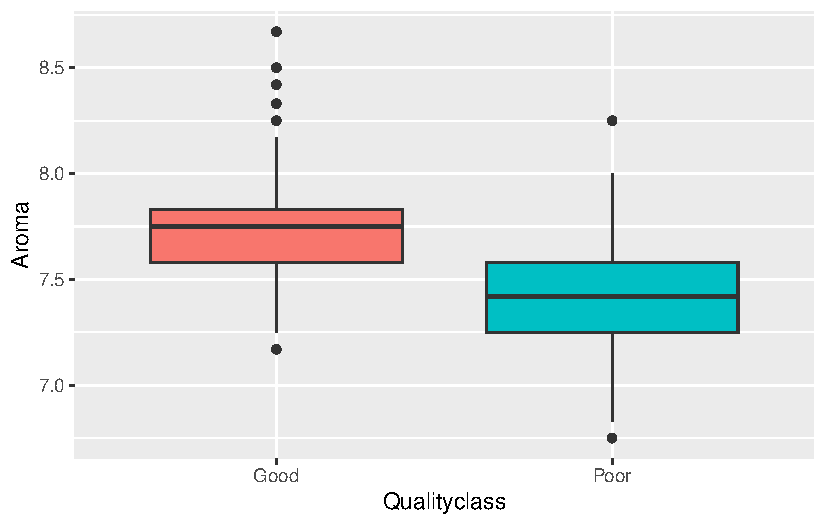
\includegraphics{project2draft_files/figure-pdf/fig-boxplot1-1.pdf}

}

\caption{\label{fig-boxplot1}Aroma Grade by Coffee Quality Class}

\end{figure}%

In Figure~\ref{fig-boxplot1}, the boxplot displays the distribution of
the Aroma scores for coffee samples categorized into two quality
classes: Good and Poor. The median aroma score for the Good quality
class is higher than that of the Poor quality class, indicating that
coffee samples classified as good tend to have better aroma ratings. The
IQR (the length of the box) is similar for both quality classes,
suggesting comparable variability in aroma scores within each category.
The spread of aroma ratings is slightly wider for Poor quality coffee
compared to Good coffee. The Good quality class has a few high aroma
outliers above 8.5, whereas the Poor class has some lower outliers near
7.0. In conclusion, coffee samples with a Good quality classification
generally exhibit higher aroma ratings, whereas Poor quality samples
tend to have lower median scores and slightly higher variability.

\begin{Shaded}
\begin{Highlighting}[]
\FunctionTok{ggplot}\NormalTok{(}\AttributeTok{data =}\NormalTok{ coffee1, }\FunctionTok{aes}\NormalTok{(}\AttributeTok{x=}\NormalTok{Qualityclass, }
                           \AttributeTok{y =}\NormalTok{ flavor, }
                           \AttributeTok{fill=}\NormalTok{Qualityclass))}\SpecialCharTok{+}
  \FunctionTok{geom\_boxplot}\NormalTok{()}\SpecialCharTok{+}
  \FunctionTok{labs}\NormalTok{(}\AttributeTok{x =} \StringTok{"Qualityclass"}\NormalTok{, }\AttributeTok{y =} \StringTok{"Flavor"}\NormalTok{)}\SpecialCharTok{+}
  \FunctionTok{theme}\NormalTok{(}\AttributeTok{legend.position =} \StringTok{"none"}\NormalTok{)}
\end{Highlighting}
\end{Shaded}

\begin{figure}[H]

\centering{

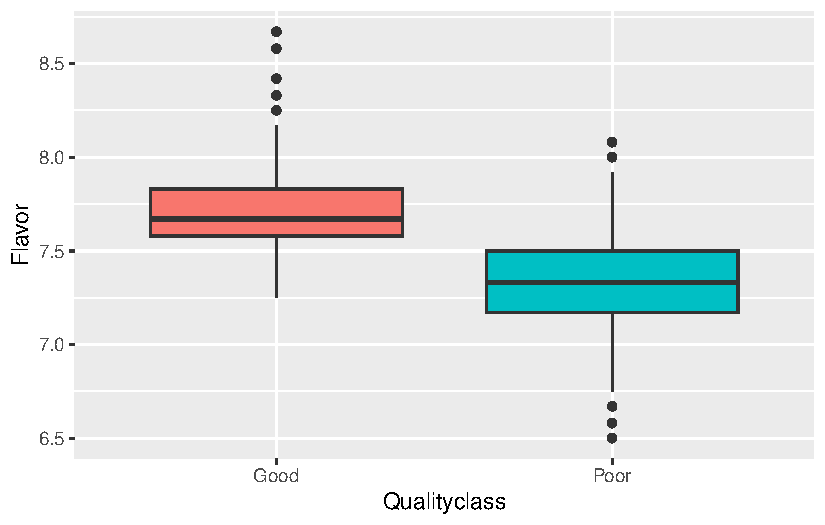
\includegraphics{project2draft_files/figure-pdf/fig-boxplot2-1.pdf}

}

\caption{\label{fig-boxplot2}Flavor Grade by Coffee Quality Class}

\end{figure}%

In Figure~\ref{fig-boxplot2}, the boxplot illustrates the distribution
of Flavor scores for coffee samples categorized as either Good or Poor
quality.The median flavor score for the Good quality class is noticeably
higher than that of the Poor class, suggesting that coffee samples
classified as Good tend to have better flavor ratings on average. The
IQR (box length) for Good quality coffee is slightly smaller than that
of Poor quality coffee, indicating that the flavor ratings are more
consistent within the Good category. The Poor quality class exhibits a
wider spread in scores, indicating greater variability in flavor
ratings. Both quality classes have several outliers, with Good quality
coffee having high-value outliers above 8.5. The Poor category has more
outliers on the lower end, with flavor scores dropping below 6.5. In
conclusion, coffee samples in the Good quality class generally receive
higher flavor ratings than those in the Poor class. The Poor quality
coffee exhibits greater variability in flavor, with some samples scoring
significantly lower.

\begin{Shaded}
\begin{Highlighting}[]
\FunctionTok{ggplot}\NormalTok{(}\AttributeTok{data =}\NormalTok{ coffee1, }\FunctionTok{aes}\NormalTok{(}\AttributeTok{x=}\NormalTok{Qualityclass, }
                           \AttributeTok{y =}\NormalTok{ acidity, }
                           \AttributeTok{fill=}\NormalTok{Qualityclass))}\SpecialCharTok{+}
  \FunctionTok{geom\_boxplot}\NormalTok{()}\SpecialCharTok{+}
  \FunctionTok{labs}\NormalTok{(}\AttributeTok{x =} \StringTok{"Qualityclass"}\NormalTok{, }\AttributeTok{y =} \StringTok{"Acidity"}\NormalTok{)}\SpecialCharTok{+}
  \FunctionTok{theme}\NormalTok{(}\AttributeTok{legend.position =} \StringTok{"none"}\NormalTok{)}
\end{Highlighting}
\end{Shaded}

\begin{figure}[H]

\centering{

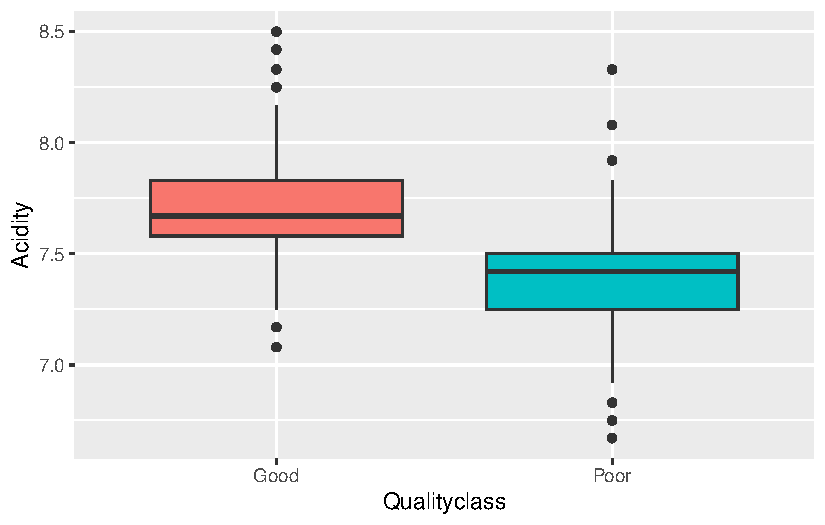
\includegraphics{project2draft_files/figure-pdf/fig-boxplot3-1.pdf}

}

\caption{\label{fig-boxplot3}Acidity Grade by Coffee Quality Class}

\end{figure}%

In Figure~\ref{fig-boxplot3}, the boxplot illustrates the distribution
of Acidity scores for coffee samples categorized as either Good or Poor
quality. The median acidity score for the Good quality class is higher
than that of the Poor quality class, suggesting that coffee samples
classified as Good generally have higher acidity ratings, which may
contribute to a brighter and more desirable flavor profile. The IQR (box
length) for both Good and Poor quality classes appears similar,
indicating comparable variability in acidity scores. However, Good
quality coffee seems to have a slightly more compact distribution,
implying more consistency in acidity ratings. Both classes have several
outliers, but Good quality coffee has more outliers above 8.0, while
Poor quality coffee has more outliers below 7.0. This suggests that some
poor-quality coffee samples have notably lower acidity scores, while
some good-quality samples exhibit particularly high acidity. In
conclusion, coffee samples classified as Good generally have higher and
more consistent acidity ratings compared to Poor quality samples, which
shows greater variability and lower acidity scores.

\begin{Shaded}
\begin{Highlighting}[]
\FunctionTok{ggplot}\NormalTok{(}\AttributeTok{data =}\NormalTok{ coffee1, }\FunctionTok{aes}\NormalTok{(}\AttributeTok{x=}\NormalTok{Qualityclass, }
                           \AttributeTok{y =}\NormalTok{ category\_two\_defects, }
                           \AttributeTok{fill=}\NormalTok{Qualityclass))}\SpecialCharTok{+}
  \FunctionTok{geom\_boxplot}\NormalTok{()}\SpecialCharTok{+}
  \FunctionTok{labs}\NormalTok{(}\AttributeTok{x =} \StringTok{"Qualityclass"}\NormalTok{, }\AttributeTok{y =} \StringTok{"Category\_two\_defects"}\NormalTok{)}\SpecialCharTok{+}
  \FunctionTok{theme}\NormalTok{(}\AttributeTok{legend.position =} \StringTok{"none"}\NormalTok{)}
\end{Highlighting}
\end{Shaded}

\begin{figure}[H]

\centering{

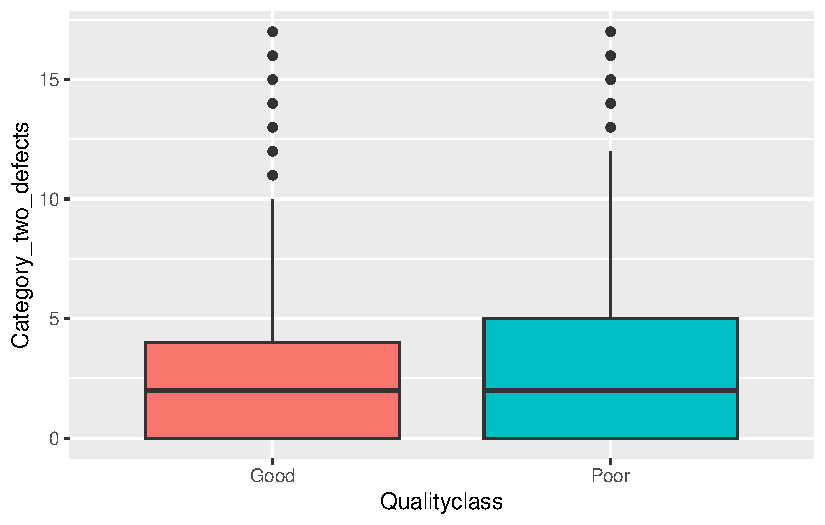
\includegraphics{project2draft_files/figure-pdf/fig-boxplot4-1.pdf}

}

\caption{\label{fig-boxplot4}Count of two Category defects by Coffee
Quality Class}

\end{figure}%

In Figure~\ref{fig-boxplot4}, The boxplot visualizes the distribution of
Category Two Defects across different Coffee Quality Classes (Good and
Poor). The median number of defects is slightly higher for the Poor
quality class compared to the Good quality class, suggests that higher
defect counts are more commonly associated with lower-quality coffee.
Both quality classes have a similar IQR (box length), meaning the
variability in defect counts within each category is comparable. The
Poor quality class exhibits a slightly wider spread, indicating a
greater range of defect occurrences. Both quality classes contain
numerous outliers, but Poor quality coffee has more extreme values, with
defect counts exceeding 15. In conclusion, poor quality coffee generally
has a higher number of defects than Good quality coffee. However,
defects are not entirely absent in Good quality coffee, as some samples
still exhibit minor defects.

\begin{Shaded}
\begin{Highlighting}[]
\FunctionTok{ggplot}\NormalTok{(}\AttributeTok{data =}\NormalTok{ coffee1, }\FunctionTok{aes}\NormalTok{(}\AttributeTok{x=}\NormalTok{Qualityclass, }
                           \AttributeTok{y =}\NormalTok{ altitude\_mean\_meters, }
                           \AttributeTok{fill=}\NormalTok{Qualityclass))}\SpecialCharTok{+}
  \FunctionTok{geom\_boxplot}\NormalTok{()}\SpecialCharTok{+}
  \FunctionTok{labs}\NormalTok{(}\AttributeTok{x =} \StringTok{"Qualityclass"}\NormalTok{, }\AttributeTok{y =} \StringTok{"Altitude (by meters)"}\NormalTok{)}\SpecialCharTok{+}
  \FunctionTok{theme}\NormalTok{(}\AttributeTok{legend.position =} \StringTok{"none"}\NormalTok{)}
\end{Highlighting}
\end{Shaded}

\begin{figure}[H]

\centering{

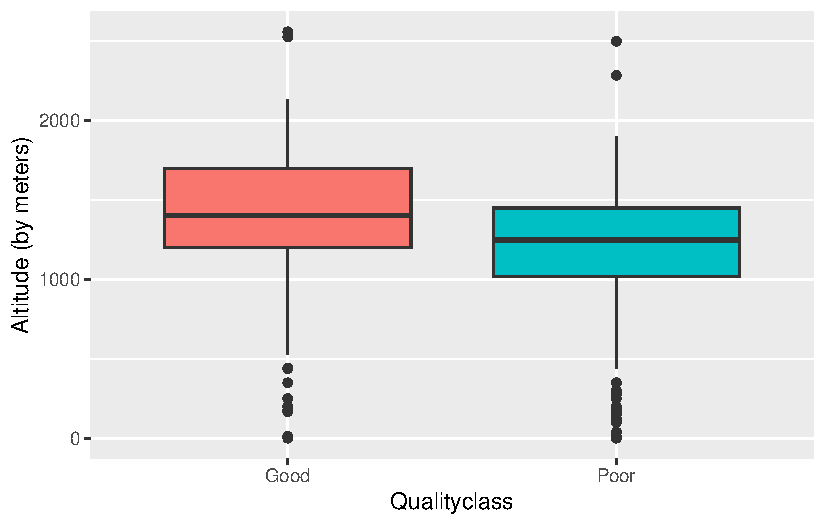
\includegraphics{project2draft_files/figure-pdf/fig-boxplot5-1.pdf}

}

\caption{\label{fig-boxplot5}Mean Altitude (in meters) by Coffee Quality
Class}

\end{figure}%

In Figure~\ref{fig-boxplot5}, boxplot visualizes the distribution of
mean altitude (in meters) for coffee samples classified into Good and
Poor quality classes. The median altitude for the Good quality class is
slightly higher than that of the Poor quality class. Both quality
classes exhibit similar IQRs (box lengths), indicating comparable
variability in growing altitudes. However, the Good quality class
appears to have a higher overall distribution of altitude values. Both
quality classes contain multiple outliers, but the Poor quality class
has more extreme low-altitude values. In conclusion, good quality coffee
is generally associated with higher altitude cultivation, while Poor
quality coffee includes more low-altitude samples and exhibits greater
variability.

\begin{Shaded}
\begin{Highlighting}[]
\FunctionTok{ggplot}\NormalTok{(}\AttributeTok{data =}\NormalTok{ coffee1, }\FunctionTok{aes}\NormalTok{(}\AttributeTok{x=}\NormalTok{Qualityclass, }
                           \AttributeTok{y =}\NormalTok{ harvested, }
                           \AttributeTok{fill=}\NormalTok{Qualityclass))}\SpecialCharTok{+}
  \FunctionTok{geom\_boxplot}\NormalTok{()}\SpecialCharTok{+}
  \FunctionTok{labs}\NormalTok{(}\AttributeTok{x =} \StringTok{"Qualityclass"}\NormalTok{, }\AttributeTok{y =} \StringTok{"Harvested Year"}\NormalTok{)}\SpecialCharTok{+}
  \FunctionTok{theme}\NormalTok{(}\AttributeTok{legend.position =} \StringTok{"none"}\NormalTok{)}
\end{Highlighting}
\end{Shaded}

\begin{figure}[H]

\centering{

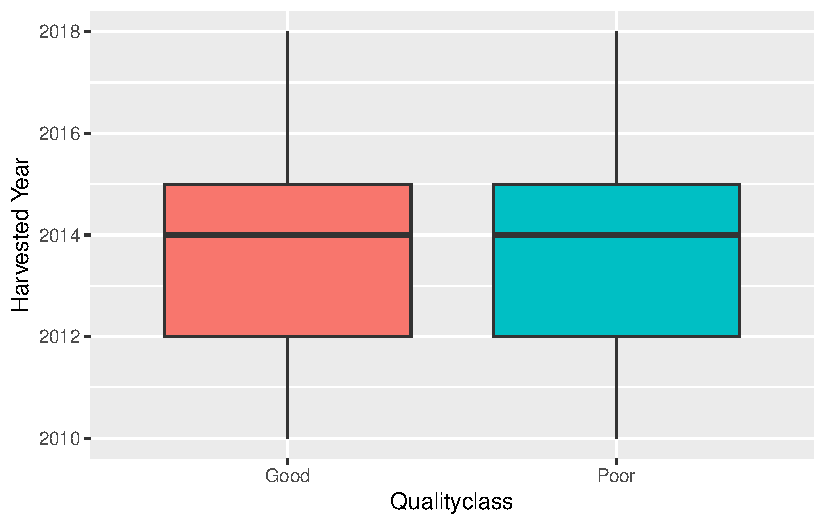
\includegraphics{project2draft_files/figure-pdf/fig-boxplot6-1.pdf}

}

\caption{\label{fig-boxplot6}Harvested Year by Coffee Quality Class}

\end{figure}%

In Figure~\ref{fig-boxplot6}, this boxplot visualizes the distribution
of harvested years for coffee samples categorized as Good and Poor
quality classes. The median harvested year for both Good and Poor
quality classes appears to be similar, around 2014, suggesting that
coffee quality may not be strongly influenced by the harvest year within
this dataset. The IQRs (box lengths) are nearly identical, indicating
that both quality classes have a similar spread of harvested years. The
typical harvest years for both Good and Poor quality coffee range
approximately from 2012 to 2016. There do not appear to be significant
outliers, suggesting a relatively consistent harvest time distribution
across quality classes. In conclusion, harvest year does not appear to
be a key determinant of coffee quality in this dataset. \# Formal
Analysis

\subsection{Model Fitting}\label{model-fitting}

\begin{Shaded}
\begin{Highlighting}[]
\CommentTok{\# Fit GLM model.}
\NormalTok{model }\OtherTok{\textless{}{-}} \FunctionTok{glm}\NormalTok{(}\AttributeTok{formula=}\NormalTok{Qualityclass}\SpecialCharTok{\textasciitilde{}}\NormalTok{ aroma }\SpecialCharTok{+}\NormalTok{ flavor }\SpecialCharTok{+}\NormalTok{ acidity }\SpecialCharTok{+}
\NormalTok{               category\_two\_defects }\SpecialCharTok{+} 
\NormalTok{               altitude\_mean\_meters }\SpecialCharTok{+} 
\NormalTok{               harvested,}
             \AttributeTok{data =}\NormalTok{ coffee1,}
             \AttributeTok{family =} \FunctionTok{binomial}\NormalTok{(}\AttributeTok{link =} \StringTok{"logit"}\NormalTok{))}
\end{Highlighting}
\end{Shaded}

\begin{Shaded}
\begin{Highlighting}[]
\CommentTok{\# check for the baseline category response variable}
\FunctionTok{levels}\NormalTok{(coffee1}\SpecialCharTok{$}\NormalTok{Qualityclass)}
\end{Highlighting}
\end{Shaded}

\begin{verbatim}
[1] "Good" "Poor"
\end{verbatim}

Note in this example, the baseline category for binary response
(Qualityclass) is \emph{Good}.

\begin{Shaded}
\begin{Highlighting}[]
\CommentTok{\# Summary statistics}
\FunctionTok{summ}\NormalTok{(model)}
\end{Highlighting}
\end{Shaded}

\begin{table}[!h]
\centering
\begin{tabular}{lr}
\toprule
\cellcolor{gray!10}{Observations} & \cellcolor{gray!10}{882}\\
Dependent variable & Qualityclass\\
\cellcolor{gray!10}{Type} & \cellcolor{gray!10}{Generalized linear model}\\
Family & binomial\\
\cellcolor{gray!10}{Link} & \cellcolor{gray!10}{logit}\\
\bottomrule
\end{tabular}
\end{table} \begin{table}[!h]
\centering
\begin{tabular}{lr}
\toprule
\cellcolor{gray!10}{$\chi^2$(6)} & \cellcolor{gray!10}{688.21}\\
p & 0.00\\
\cellcolor{gray!10}{Pseudo-R² (Cragg-Uhler)} & \cellcolor{gray!10}{0.72}\\
Pseudo-R² (McFadden) & 0.56\\
\cellcolor{gray!10}{AIC} & \cellcolor{gray!10}{547.34}\\
\addlinespace
BIC & 580.82\\
\bottomrule
\end{tabular}
\end{table} \begin{table}[!h]
\centering
\begin{threeparttable}
\begin{tabular}{lrrrr}
\toprule
  & Est. & S.E. & z val. & p\\
\midrule
\cellcolor{gray!10}{(Intercept)} & \cellcolor{gray!10}{313.21} & \cellcolor{gray!10}{120.90} & \cellcolor{gray!10}{2.59} & \cellcolor{gray!10}{0.01}\\
aroma & -4.64 & 0.72 & -6.46 & 0.00\\
\cellcolor{gray!10}{flavor} & \cellcolor{gray!10}{-7.09} & \cellcolor{gray!10}{0.87} & \cellcolor{gray!10}{-8.17} & \cellcolor{gray!10}{0.00}\\
acidity & -4.13 & 0.68 & -6.09 & 0.00\\
\cellcolor{gray!10}{category\_two\_defects} & \cellcolor{gray!10}{0.00} & \cellcolor{gray!10}{0.03} & \cellcolor{gray!10}{0.00} & \cellcolor{gray!10}{1.00}\\
\addlinespace
altitude\_mean\_meters & -0.00 & 0.00 & -3.13 & 0.00\\
\cellcolor{gray!10}{harvested} & \cellcolor{gray!10}{-0.10} & \cellcolor{gray!10}{0.06} & \cellcolor{gray!10}{-1.61} & \cellcolor{gray!10}{0.11}\\
\bottomrule
\end{tabular}
\begin{tablenotes}
\item Standard errors: MLE
\end{tablenotes}
\end{threeparttable}
\end{table}

The model suggests that Aroma, Flavor, and Acidity are the most
important factors in determining coffee quality. Harvested Year is also
not significant (p = 0.11), suggesting that coffee quality
classification does not strongly depend on the year it was harvested.
Note that the explanatory variable category\_two\_defects has a p-value
of 1, which is not significant at all. Consequently, it should not be
considered for the further analysis and should be removed initially.

\begin{Shaded}
\begin{Highlighting}[]
\CommentTok{\# Model with one variable dropped.}
\NormalTok{model2 }\OtherTok{\textless{}{-}} \FunctionTok{glm}\NormalTok{(}\AttributeTok{formula =}\NormalTok{ Qualityclass}\SpecialCharTok{\textasciitilde{}}\NormalTok{ aroma }\SpecialCharTok{+}\NormalTok{ flavor }\SpecialCharTok{+}\NormalTok{ acidity }\SpecialCharTok{+}
\NormalTok{               altitude\_mean\_meters }\SpecialCharTok{+} 
\NormalTok{               harvested,}
             \AttributeTok{data =}\NormalTok{ coffee1,}
             \AttributeTok{family =} \FunctionTok{binomial}\NormalTok{(}\AttributeTok{link =} \StringTok{"logit"}\NormalTok{))}

\FunctionTok{summ}\NormalTok{(model2)}
\end{Highlighting}
\end{Shaded}

\begin{table}[!h]
\centering
\begin{tabular}{lr}
\toprule
\cellcolor{gray!10}{Observations} & \cellcolor{gray!10}{882}\\
Dependent variable & Qualityclass\\
\cellcolor{gray!10}{Type} & \cellcolor{gray!10}{Generalized linear model}\\
Family & binomial\\
\cellcolor{gray!10}{Link} & \cellcolor{gray!10}{logit}\\
\bottomrule
\end{tabular}
\end{table} \begin{table}[!h]
\centering
\begin{tabular}{lr}
\toprule
\cellcolor{gray!10}{$\chi^2$(5)} & \cellcolor{gray!10}{688.21}\\
p & 0.00\\
\cellcolor{gray!10}{Pseudo-R² (Cragg-Uhler)} & \cellcolor{gray!10}{0.72}\\
Pseudo-R² (McFadden) & 0.56\\
\cellcolor{gray!10}{AIC} & \cellcolor{gray!10}{545.34}\\
\addlinespace
BIC & 574.04\\
\bottomrule
\end{tabular}
\end{table} \begin{table}[!h]
\centering
\begin{threeparttable}
\begin{tabular}{lrrrr}
\toprule
  & Est. & S.E. & z val. & p\\
\midrule
\cellcolor{gray!10}{(Intercept)} & \cellcolor{gray!10}{313.21} & \cellcolor{gray!10}{120.41} & \cellcolor{gray!10}{2.60} & \cellcolor{gray!10}{0.01}\\
aroma & -4.64 & 0.72 & -6.46 & 0.00\\
\cellcolor{gray!10}{flavor} & \cellcolor{gray!10}{-7.09} & \cellcolor{gray!10}{0.87} & \cellcolor{gray!10}{-8.17} & \cellcolor{gray!10}{0.00}\\
acidity & -4.13 & 0.68 & -6.09 & 0.00\\
\cellcolor{gray!10}{altitude\_mean\_meters} & \cellcolor{gray!10}{-0.00} & \cellcolor{gray!10}{0.00} & \cellcolor{gray!10}{-3.14} & \cellcolor{gray!10}{0.00}\\
\addlinespace
harvested & -0.10 & 0.06 & -1.61 & 0.11\\
\bottomrule
\end{tabular}
\begin{tablenotes}
\item Standard errors: MLE
\end{tablenotes}
\end{threeparttable}
\end{table}

The model remains strong and statistically valid, with Aroma, Flavor,
and Acidity being the strongest predictors of coffee quality. Altitude
is statistically significant but has a minimal effect, meaning it may
not be a primary determinant of quality. The model fit (AIC/BIC)
decreased, indicating that removing insignificant variables does not
impact predictive power. Assuming a p-value of 0.05, harvested Year (p =
0.11) remains not statistically significant, meaning coffee quality is
not strongly dependent on the year of harvest, an attempt was made to
remove the only non-significant variable, harvested.

\begin{Shaded}
\begin{Highlighting}[]
\NormalTok{model3 }\OtherTok{\textless{}{-}} \FunctionTok{glm}\NormalTok{(}\AttributeTok{formula =}\NormalTok{ Qualityclass}\SpecialCharTok{\textasciitilde{}}\NormalTok{ aroma }\SpecialCharTok{+}\NormalTok{ flavor }\SpecialCharTok{+}\NormalTok{ acidity }\SpecialCharTok{+}
\NormalTok{               altitude\_mean\_meters,}
             \AttributeTok{data =}\NormalTok{ coffee1,}
             \AttributeTok{family =} \FunctionTok{binomial}\NormalTok{(}\AttributeTok{link =} \StringTok{"logit"}\NormalTok{))}

\FunctionTok{summ}\NormalTok{(model3)}
\end{Highlighting}
\end{Shaded}

\begin{table}[!h]
\centering
\begin{tabular}{lr}
\toprule
\cellcolor{gray!10}{Observations} & \cellcolor{gray!10}{882}\\
Dependent variable & Qualityclass\\
\cellcolor{gray!10}{Type} & \cellcolor{gray!10}{Generalized linear model}\\
Family & binomial\\
\cellcolor{gray!10}{Link} & \cellcolor{gray!10}{logit}\\
\bottomrule
\end{tabular}
\end{table} \begin{table}[!h]
\centering
\begin{tabular}{lr}
\toprule
\cellcolor{gray!10}{$\chi^2$(4)} & \cellcolor{gray!10}{685.59}\\
p & 0.00\\
\cellcolor{gray!10}{Pseudo-R² (Cragg-Uhler)} & \cellcolor{gray!10}{0.72}\\
Pseudo-R² (McFadden) & 0.56\\
\cellcolor{gray!10}{AIC} & \cellcolor{gray!10}{545.96}\\
\addlinespace
BIC & 569.87\\
\bottomrule
\end{tabular}
\end{table} \begin{table}[!h]
\centering
\begin{threeparttable}
\begin{tabular}{lrrrr}
\toprule
  & Est. & S.E. & z val. & p\\
\midrule
\cellcolor{gray!10}{(Intercept)} & \cellcolor{gray!10}{120.10} & \cellcolor{gray!10}{8.73} & \cellcolor{gray!10}{13.76} & \cellcolor{gray!10}{0.00}\\
aroma & -4.50 & 0.71 & -6.36 & 0.00\\
\cellcolor{gray!10}{flavor} & \cellcolor{gray!10}{-7.08} & \cellcolor{gray!10}{0.87} & \cellcolor{gray!10}{-8.18} & \cellcolor{gray!10}{0.00}\\
acidity & -4.20 & 0.68 & -6.19 & 0.00\\
\cellcolor{gray!10}{altitude\_mean\_meters} & \cellcolor{gray!10}{-0.00} & \cellcolor{gray!10}{0.00} & \cellcolor{gray!10}{-2.92} & \cellcolor{gray!10}{0.00}\\
\bottomrule
\end{tabular}
\begin{tablenotes}
\item Standard errors: MLE
\end{tablenotes}
\end{threeparttable}
\end{table}

All Remaining Variables Are Statistically Significant (p \textless{}
0.05): Aroma, Flavor, and Acidity remain the strongest predictors, with
higher values correlating with better coffee quality; Altitude is still
significant, but its effect size is very small. The AIC of model 3 is
observed to increase a little following the removal of the variable
harvested, but the BIC decrease as expected. Consequently, model 3 is
deemed to be the most suitable.

\begin{Shaded}
\begin{Highlighting}[]
\CommentTok{\# Fit GLM model including all variables.}
\NormalTok{coffee1}\SpecialCharTok{$}\NormalTok{country\_of\_origin }\OtherTok{\textless{}{-}} \FunctionTok{as.factor}\NormalTok{(coffee1}\SpecialCharTok{$}\NormalTok{country\_of\_origin)}
\NormalTok{glm\_model }\OtherTok{\textless{}{-}} \FunctionTok{glm}\NormalTok{(Qualityclass }\SpecialCharTok{\textasciitilde{}}\NormalTok{ .,}
                 \AttributeTok{data =}\NormalTok{ coffee1,}
                 \AttributeTok{family =} \FunctionTok{binomial}\NormalTok{(}\AttributeTok{link =} \StringTok{"logit"}\NormalTok{))}
\FunctionTok{summ}\NormalTok{(glm\_model)}
\end{Highlighting}
\end{Shaded}

\begin{table}[!h]
\centering
\begin{tabular}{lr}
\toprule
\cellcolor{gray!10}{Observations} & \cellcolor{gray!10}{882}\\
Dependent variable & Qualityclass\\
\cellcolor{gray!10}{Type} & \cellcolor{gray!10}{Generalized linear model}\\
Family & binomial\\
\cellcolor{gray!10}{Link} & \cellcolor{gray!10}{logit}\\
\bottomrule
\end{tabular}
\end{table} \begin{table}[!h]
\centering
\begin{tabular}{lr}
\toprule
\cellcolor{gray!10}{$\chi^2$(38)} & \cellcolor{gray!10}{774.22}\\
p & 0.00\\
\cellcolor{gray!10}{Pseudo-R² (Cragg-Uhler)} & \cellcolor{gray!10}{0.78}\\
Pseudo-R² (McFadden) & 0.63\\
\cellcolor{gray!10}{AIC} & \cellcolor{gray!10}{525.33}\\
\addlinespace
BIC & 711.84\\
\bottomrule
\end{tabular}
\end{table} \begin{table}[!h]
\centering
\begin{threeparttable}
\begin{tabular}{lrrrr}
\toprule
  & Est. & S.E. & z val. & p\\
\midrule
\cellcolor{gray!10}{(Intercept)} & \cellcolor{gray!10}{417.93} & \cellcolor{gray!10}{155.81} & \cellcolor{gray!10}{2.68} & \cellcolor{gray!10}{0.01}\\
country\_of\_originBurundi & -1.74 & 4.94 & -0.35 & 0.72\\
\cellcolor{gray!10}{country\_of\_originChina} & \cellcolor{gray!10}{0.20} & \cellcolor{gray!10}{1.02} & \cellcolor{gray!10}{0.19} & \cellcolor{gray!10}{0.85}\\
country\_of\_originColombia & -1.68 & 0.56 & -3.02 & 0.00\\
\cellcolor{gray!10}{country\_of\_originCosta Rica} & \cellcolor{gray!10}{0.03} & \cellcolor{gray!10}{0.71} & \cellcolor{gray!10}{0.05} & \cellcolor{gray!10}{0.96}\\
\addlinespace
country\_of\_originCote d?Ivoire & 11.18 & 3956.18 & 0.00 & 1.00\\
\cellcolor{gray!10}{country\_of\_originEcuador} & \cellcolor{gray!10}{1.20} & \cellcolor{gray!10}{1.48} & \cellcolor{gray!10}{0.81} & \cellcolor{gray!10}{0.42}\\
country\_of\_originEl Salvador & -0.26 & 0.94 & -0.27 & 0.78\\
\cellcolor{gray!10}{country\_of\_originEthiopia} & \cellcolor{gray!10}{-10.89} & \cellcolor{gray!10}{646.51} & \cellcolor{gray!10}{-0.02} & \cellcolor{gray!10}{0.99}\\
country\_of\_originGuatemala & 0.82 & 0.51 & 1.61 & 0.11\\
\addlinespace
\cellcolor{gray!10}{country\_of\_originHaiti} & \cellcolor{gray!10}{-2.10} & \cellcolor{gray!10}{1.87} & \cellcolor{gray!10}{-1.12} & \cellcolor{gray!10}{0.26}\\
country\_of\_originHonduras & 0.79 & 0.65 & 1.21 & 0.23\\
\cellcolor{gray!10}{country\_of\_originIndia} & \cellcolor{gray!10}{3.82} & \cellcolor{gray!10}{1.22} & \cellcolor{gray!10}{3.14} & \cellcolor{gray!10}{0.00}\\
country\_of\_originIndonesia & 0.55 & 0.91 & 0.61 & 0.54\\
\cellcolor{gray!10}{country\_of\_originKenya} & \cellcolor{gray!10}{-0.61} & \cellcolor{gray!10}{1.45} & \cellcolor{gray!10}{-0.42} & \cellcolor{gray!10}{0.67}\\
\addlinespace
country\_of\_originLaos & 14.68 & 2674.02 & 0.01 & 1.00\\
\cellcolor{gray!10}{country\_of\_originMalawi} & \cellcolor{gray!10}{1.35} & \cellcolor{gray!10}{1.23} & \cellcolor{gray!10}{1.09} & \cellcolor{gray!10}{0.27}\\
country\_of\_originMauritius & 11.12 & 3956.18 & 0.00 & 1.00\\
\cellcolor{gray!10}{country\_of\_originMexico} & \cellcolor{gray!10}{0.87} & \cellcolor{gray!10}{0.48} & \cellcolor{gray!10}{1.83} & \cellcolor{gray!10}{0.07}\\
country\_of\_originMyanmar & 14.94 & 2797.24 & 0.01 & 1.00\\
\addlinespace
\cellcolor{gray!10}{country\_of\_originNicaragua} & \cellcolor{gray!10}{-0.13} & \cellcolor{gray!10}{1.82} & \cellcolor{gray!10}{-0.07} & \cellcolor{gray!10}{0.94}\\
country\_of\_originPanama & -2.92 & 1.72 & -1.70 & 0.09\\
\cellcolor{gray!10}{country\_of\_originPeru} & \cellcolor{gray!10}{13.57} & \cellcolor{gray!10}{3956.18} & \cellcolor{gray!10}{0.00} & \cellcolor{gray!10}{1.00}\\
country\_of\_originPhilippines & -2.29 & 2.82 & -0.81 & 0.42\\
\cellcolor{gray!10}{country\_of\_originTaiwan} & \cellcolor{gray!10}{-0.50} & \cellcolor{gray!10}{0.62} & \cellcolor{gray!10}{-0.81} & \cellcolor{gray!10}{0.42}\\
\addlinespace
country\_of\_originTanzania, United Republic Of & -0.71 & 0.73 & -0.97 & 0.33\\
\cellcolor{gray!10}{country\_of\_originThailand} & \cellcolor{gray!10}{-2.17} & \cellcolor{gray!10}{0.96} & \cellcolor{gray!10}{-2.26} & \cellcolor{gray!10}{0.02}\\
country\_of\_originUganda & 1.66 & 0.76 & 2.17 & 0.03\\
\cellcolor{gray!10}{country\_of\_originUnited States} & \cellcolor{gray!10}{-1.67} & \cellcolor{gray!10}{1.77} & \cellcolor{gray!10}{-0.94} & \cellcolor{gray!10}{0.35}\\
country\_of\_originUnited States (Hawaii) & -3.73 & 3956.18 & -0.00 & 1.00\\
\addlinespace
\cellcolor{gray!10}{country\_of\_originUnited States (Puerto Rico)} & \cellcolor{gray!10}{2.91} & \cellcolor{gray!10}{1.66} & \cellcolor{gray!10}{1.75} & \cellcolor{gray!10}{0.08}\\
country\_of\_originVietnam & -1.71 & 1.10 & -1.55 & 0.12\\
\cellcolor{gray!10}{country\_of\_originZambia} & \cellcolor{gray!10}{13.40} & \cellcolor{gray!10}{3956.18} & \cellcolor{gray!10}{0.00} & \cellcolor{gray!10}{1.00}\\
aroma & -5.30 & 0.85 & -6.25 & 0.00\\
\cellcolor{gray!10}{flavor} & \cellcolor{gray!10}{-7.91} & \cellcolor{gray!10}{1.02} & \cellcolor{gray!10}{-7.72} & \cellcolor{gray!10}{0.00}\\
\addlinespace
acidity & -5.37 & 0.81 & -6.60 & 0.00\\
\cellcolor{gray!10}{category\_two\_defects} & \cellcolor{gray!10}{-0.06} & \cellcolor{gray!10}{0.04} & \cellcolor{gray!10}{-1.49} & \cellcolor{gray!10}{0.14}\\
altitude\_mean\_meters & -0.00 & 0.00 & -1.69 & 0.09\\
\cellcolor{gray!10}{harvested} & \cellcolor{gray!10}{-0.14} & \cellcolor{gray!10}{0.08} & \cellcolor{gray!10}{-1.80} & \cellcolor{gray!10}{0.07}\\
\bottomrule
\end{tabular}
\begin{tablenotes}
\item Standard errors: MLE
\end{tablenotes}
\end{threeparttable}
\end{table}

Significant Predictors (p \textless{} 0.05): Aroma, Flavor, and Acidity
remain highly significant, confirming their strong impact on coffee
quality. Several countries of origin (Colombia, India, Thailand, Uganda)
are statistically significant, indicating that origin may influence
coffee quality. Non-Significant Predictors (p \textgreater{} 0.05): Many
country of origin variables (e.g., Burundi, China, Ethiopia, Vietnam)
are not significant, meaning they do not strongly predict coffee
quality. Altitude, Harvest Year, and Category Two Defects remain
non-significant, suggesting they should be removed in further
refinements.

Following the incorporation of all variables into the model, an
enhancement in R square, that is to say an improvement in
interpretability, was observed, concomitant with a diminution in AIC.
However, a substantial increase was observed in the BIC, which may not
be considered a valuable gain due to the cost of adding a large number
of degrees of freedom.

\subsection{log-odds}\label{log-odds}

\begin{Shaded}
\begin{Highlighting}[]
\NormalTok{mod1coefs }\OtherTok{\textless{}{-}} \FunctionTok{round}\NormalTok{(}\FunctionTok{coef}\NormalTok{(model3),}\DecValTok{4}\NormalTok{)}
\end{Highlighting}
\end{Shaded}

\begin{align}
\ln\left(\frac{p}{1-p}\right) &= \alpha + \beta_1 \cdot \textrm{aroma} +\beta_2 \cdot \textrm{flavor} + \beta_3 \cdot \textrm{acidicity} + \beta_4 \cdot \textrm{altitude\_mean\_meters}\nonumber\\
&= 120.1024  -4.5035 \cdot \textrm{aroma}-7.0773 \cdot \textrm{flavor} -4.1992 \cdot \textrm{acidity} \ensuremath{-8\times 10^{-4}} \cdot \textrm{altitude\_mean\_meters} \nonumber
\end{align}

where \emph{p} = Prob (Quality score is \textbf{Poor}) and 1 - p =
Prob(Quality score is \textbf{Good}) as we already check and confirmed
the baseline category response is Good in the previous step.

Thus, the log-odds of the Quality score for the batch is Poor decrease
by 4.5 for every unit increase in aroma grade when hold other variables
kept unchanged. Similarly, the log-odds of the Quality score for the
batch is Poor decrease by 7.02 for every unit increase in flavor grade
when hold other variables kept unchanged. And the log-odds of the
Quality score for the batch is Poor decrease by 4.42 for every unit
increase in acidity grade when hold other variables constant.The
log-odds of a coffee batch being Poor slightly decreases as altitude
increases when hold other variables kept unchanged.

\begin{Shaded}
\begin{Highlighting}[]
\CommentTok{\# 95\% Confidence interval for the log{-}odds by different explanatory variable.}
\FunctionTok{confint}\NormalTok{(model3)}\SpecialCharTok{|\textgreater{}}
  \FunctionTok{kable}\NormalTok{()}
\end{Highlighting}
\end{Shaded}

\begin{longtable}[]{@{}lrr@{}}

\caption{\label{tbl-logoddsCI}95\% Confidence Interval for the Log-odds}

\tabularnewline

\toprule\noalign{}
& 2.5 \% & 97.5 \% \\
\midrule\noalign{}
\endhead
\bottomrule\noalign{}
\endlastfoot
(Intercept) & 103.8885588 & 138.1556953 \\
aroma & -5.9335595 & -3.1506386 \\
flavor & -8.8354161 & -5.4369193 \\
acidity & -5.5576558 & -2.8939166 \\
altitude\_mean\_meters & -0.0012911 & -0.0002563 \\

\end{longtable}

For Table~\ref{tbl-logoddsCI}, since most of the intervals don't contain
1 thus again confirmed that the explanatory variables in model 2 are
significant excluding the harvested. Flavor has the largest effect
(widest range of negative values), reinforcing its importance in coffee
quality classification. Altitude has the smallest effect size, though it
remains statistically significant.

\begin{Shaded}
\begin{Highlighting}[]
\NormalTok{mod.coef.logodds }\OtherTok{\textless{}{-}}\NormalTok{ model3 }\SpecialCharTok{|\textgreater{}}
  \FunctionTok{summary}\NormalTok{()}\SpecialCharTok{|\textgreater{}}
  \FunctionTok{coef}\NormalTok{()}
\end{Highlighting}
\end{Shaded}

\subsubsection{95\% Confidence Interval Plot For
Log-Odds}\label{confidence-interval-plot-for-log-odds}

\begin{Shaded}
\begin{Highlighting}[]
\CommentTok{\# 95\% Confidence Interval Plot for Log{-}Odds.}
\FunctionTok{plot\_model}\NormalTok{(model3, }\AttributeTok{show.values =} \ConstantTok{TRUE}\NormalTok{, }\AttributeTok{transform =} \ConstantTok{NULL}\NormalTok{,}
           \AttributeTok{title =} \StringTok{"Log{-}Odds (Poor Coffee Batch Qualtiy Score)"}\NormalTok{, }\AttributeTok{show.p =} \ConstantTok{FALSE}\NormalTok{)}
\end{Highlighting}
\end{Shaded}

\begin{figure}[H]

\centering{

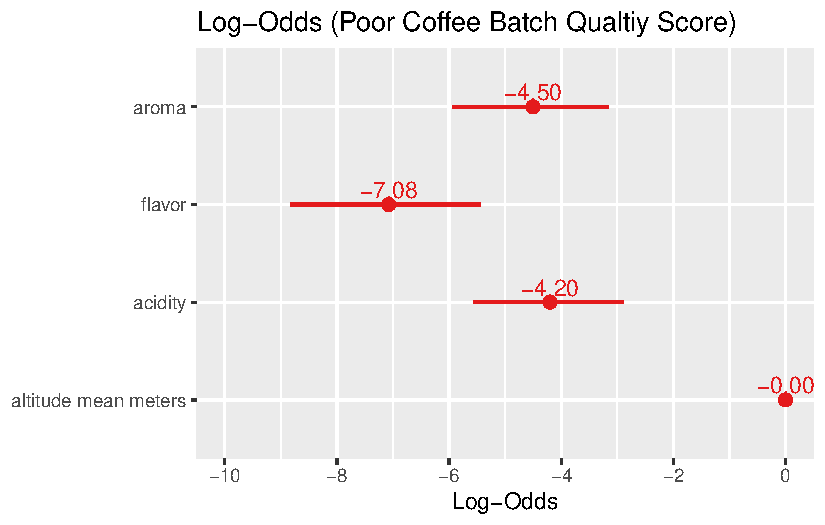
\includegraphics{project2draft_files/figure-pdf/fig-CIplot-1.pdf}

}

\caption{\label{fig-CIplot}95\% Confidence Interval Plot for Log-Odds}

\end{figure}%

\begin{Shaded}
\begin{Highlighting}[]
\CommentTok{\# Add log{-}odds to the dataset}
\NormalTok{coffee1 }\OtherTok{\textless{}{-}}\NormalTok{ coffee1 }\SpecialCharTok{|\textgreater{}}
  \FunctionTok{mutate}\NormalTok{(}\AttributeTok{logodds.poor =} \FunctionTok{predict}\NormalTok{(model3))}
\end{Highlighting}
\end{Shaded}

For Table~\ref{tbl-logoddsCI}, since most of the
intervals(\([-6.0908,-3.2701]\) for aroma grade, \([-8.8598,-5.4496]\)
for flavor grade, \([-5.4826,-2.8223]\) for acidity grade,
\([-0.0013,-0.0003]\) for altitude\_mean\_meters grade,
\([-0.2124,0.0203]\) for harvested grade), excluding the variable
harvested, don't contain zero thus indicates that the explanatory
variables in model 2 are significant. And the Figure~\ref{fig-CIplotodd}
again confirmed the significant of the explanatory variables visually.

For more straightforward interpretation, we use Odds ratio scale.

\subsection{Odds Ratio}\label{odds-ratio}

\[
\frac{p}{1-p} = \exp(\alpha + \beta_1 \cdot \textrm{aroma} +\beta_2 \cdot \textrm{flavor} + \beta_3 \cdot \textrm{acidicity})
\]

\begin{Shaded}
\begin{Highlighting}[]
\NormalTok{model3 }\SpecialCharTok{|\textgreater{}}
  \FunctionTok{coef}\NormalTok{()}\SpecialCharTok{|\textgreater{}}
  \FunctionTok{exp}\NormalTok{()}\SpecialCharTok{|\textgreater{}}
  \FunctionTok{as.data.frame}\NormalTok{()}\SpecialCharTok{|\textgreater{}}
  \FunctionTok{rownames\_to\_column}\NormalTok{(}\AttributeTok{var =} \StringTok{"Variable"}\NormalTok{)}\SpecialCharTok{|\textgreater{}}
  \FunctionTok{gt}\NormalTok{()}
\end{Highlighting}
\end{Shaded}

\begin{table}

\caption{\label{tbl-summtable}Summary Table on the Odds Scale}

\centering{

\fontsize{12.0pt}{14.4pt}\selectfont
\begin{tabular*}{\linewidth}{@{\extracolsep{\fill}}lr}
\toprule
Variable & exp(coef(model3)) \\ 
\midrule\addlinespace[2.5pt]
(Intercept) & 1.444867e+52 \\ 
aroma & 1.106983e-02 \\ 
flavor & 8.440891e-04 \\ 
acidity & 1.500796e-02 \\ 
altitude\_mean\_meters & 9.992319e-01 \\ 
\bottomrule
\end{tabular*}

}

\end{table}%

the value of the intercept (\(1.82\times10^{52}\)) gives the odds of a
quality class being poor given all explanatory variables equal to zero,
but in reality, it is highly unlikely for a batch of coffee have the
grades of aroma, flavor and acidity all approach to zero. It could still
be interpreted as when chance of a batch of coffee be classified as poor
quality are (\(1.82\times10^{52}\)) \% greater than them being
classified as good quality when all the explanatory variable equals to
zero.

For aroma grade, we have an odds of \(1.10\times10^{-2}\), which
indicates that for every 1 unit increase in aroma grade, the odds of the
quality class being poor increase by a factor of 0.01 when other
variables unchanged.

The odds for flavor grade is \(8.98\times10^{-4}\), thus the odds of the
quality class being poor increase by a factor of 0.00089 for every 1
unit increase in flavor grade,keeping all other variables constant.

Finally, the odds for acidity grade is \(1.20\times10^{-2}\), indicating
that for every 1 unit increase in acidity grade, the odds of the quality
class being poor increase by a factor of 0.012 keeping all other
variable constant.

\begin{Shaded}
\begin{Highlighting}[]
\CommentTok{\# 95\% Confidence interval for the odds by different explanatory variable.}
\FunctionTok{confint}\NormalTok{(model3) }\SpecialCharTok{|\textgreater{}}
  \FunctionTok{exp}\NormalTok{() }\SpecialCharTok{|\textgreater{}}
  \FunctionTok{kable}\NormalTok{()}
\end{Highlighting}
\end{Shaded}

\begin{longtable}[]{@{}lrr@{}}

\caption{\label{tbl-oddsCI}95\% Confidence Interval for the Odds}

\tabularnewline

\toprule\noalign{}
& 2.5 \% & 97.5 \% \\
\midrule\noalign{}
\endhead
\bottomrule\noalign{}
\endlastfoot
(Intercept) & 1.312888e+45 & 1.000590e+60 \\
aroma & 2.649000e-03 & 4.282480e-02 \\
flavor & 1.455000e-04 & 4.352900e-03 \\
acidity & 3.857800e-03 & 5.535900e-02 \\
altitude\_mean\_meters & 9.987098e-01 & 9.997437e-01 \\

\end{longtable}

\begin{Shaded}
\begin{Highlighting}[]
\FunctionTok{plot\_model}\NormalTok{(model3, }\AttributeTok{show.values =} \ConstantTok{TRUE}\NormalTok{, }
           \AttributeTok{title =} \StringTok{"Odds (Poor Quality Score)"}\NormalTok{, }\AttributeTok{show.p =} \ConstantTok{FALSE}\NormalTok{)}
\end{Highlighting}
\end{Shaded}

\begin{figure}[H]

\centering{

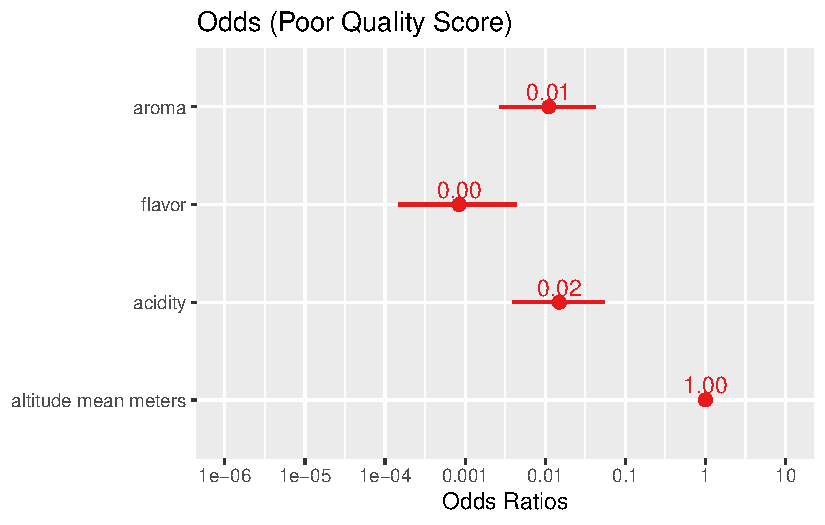
\includegraphics{project2draft_files/figure-pdf/fig-CIplotodd-1.pdf}

}

\caption{\label{fig-CIplotodd}95\% Confidence Interval Plot for Odds
Ratio}

\end{figure}%

From Table~\ref{tbl-oddsCI}, most of the intervals(\([0.0023, 0.0380]\)
for aroma grade, \([0.00014,0.0043]\) for flavor grade,
\([0.0042, 0.0594]\) for acidity grade, \([0.9986, 0.9997]\) for
altitude\_mean\_meters grade, \([0.8087, 1.0205]\) for harvested grade)
don't contain zero thus indicate that the explanatory variables in model
2 are significant.

The Figure~\ref{fig-CIplotodd} shows the 95\% confidence intervals for
three explanatory variable, again confirmed the significance of the
explanatory variables visually.

\subsection{Probability}\label{probability}

As we could obtain the probability \emph{p} = Prob (Quality score is
\textbf{Poor}) using:

\[
p = \frac{\exp(\alpha + \beta_1 \cdot \textrm{aroma} +\beta_2 \cdot \textrm{flavor} + \beta_3 \cdot \textrm{acidicity})}{1 + \exp(\alpha + \beta_1 \cdot \textrm{aroma} +\beta_2 \cdot \textrm{flavor} + \beta_3 \cdot \textrm{acidicity})}
\]

\begin{Shaded}
\begin{Highlighting}[]
\CommentTok{\# Add probability to the dataset.}
\NormalTok{coffee1 }\OtherTok{\textless{}{-}}\NormalTok{ coffee1 }\SpecialCharTok{|\textgreater{}}
  \FunctionTok{mutate}\NormalTok{(}\AttributeTok{probs.poor =} \FunctionTok{fitted}\NormalTok{(model3))}
\end{Highlighting}
\end{Shaded}

\begin{Shaded}
\begin{Highlighting}[]
\FunctionTok{ggplot}\NormalTok{(}\AttributeTok{data =}\NormalTok{ coffee1, }\FunctionTok{aes}\NormalTok{(}\AttributeTok{x =}\NormalTok{ aroma, }\AttributeTok{y =}\NormalTok{ probs.poor)) }\SpecialCharTok{+}
  \FunctionTok{geom\_smooth}\NormalTok{(}\AttributeTok{method=}\StringTok{"glm"}\NormalTok{, }
              \AttributeTok{method.args =} \FunctionTok{list}\NormalTok{(}\AttributeTok{family=}\StringTok{"binomial"}\NormalTok{), }
              \AttributeTok{se =} \ConstantTok{FALSE}\NormalTok{) }\SpecialCharTok{+}
  \FunctionTok{labs}\NormalTok{(}\AttributeTok{x =} \StringTok{"Aroma Grade"}\NormalTok{, }
       \AttributeTok{y =} \StringTok{"Probability of Quality Score is Poor by Aroma Grade"}\NormalTok{)}
\end{Highlighting}
\end{Shaded}

\begin{figure}[H]

\centering{

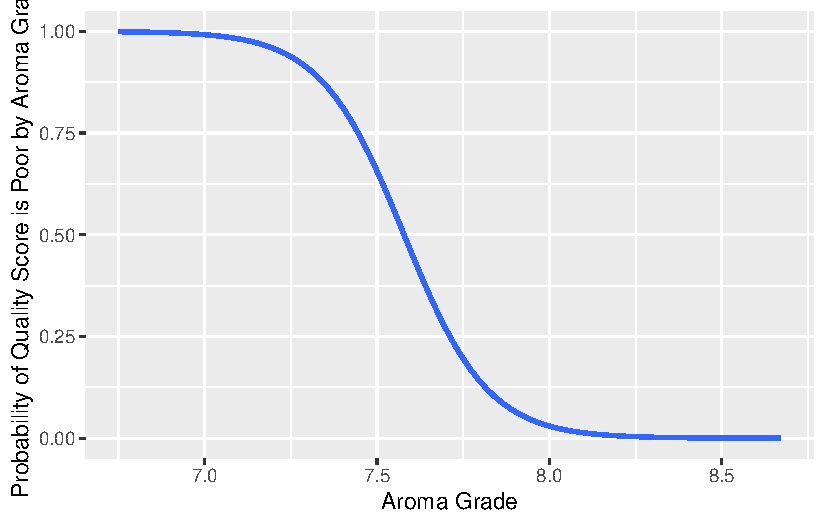
\includegraphics{project2draft_files/figure-pdf/fig-prob1-1.pdf}

}

\caption{\label{fig-prob1}Probability of Quality Score is Poor by Aroma
Grade.}

\end{figure}%

\begin{Shaded}
\begin{Highlighting}[]
\FunctionTok{ggplot}\NormalTok{(}\AttributeTok{data =}\NormalTok{ coffee1, }\FunctionTok{aes}\NormalTok{(}\AttributeTok{x =}\NormalTok{ flavor, }\AttributeTok{y =}\NormalTok{ probs.poor)) }\SpecialCharTok{+}
  \FunctionTok{geom\_smooth}\NormalTok{(}\AttributeTok{method=}\StringTok{"glm"}\NormalTok{, }
              \AttributeTok{method.args =} \FunctionTok{list}\NormalTok{(}\AttributeTok{family=}\StringTok{"binomial"}\NormalTok{), }
              \AttributeTok{se =} \ConstantTok{FALSE}\NormalTok{) }\SpecialCharTok{+}
  \FunctionTok{labs}\NormalTok{(}\AttributeTok{x =} \StringTok{"Flavor Grade"}\NormalTok{, }
       \AttributeTok{y =} \StringTok{"Probability of Quality Score is Poor by Flavor Grade"}\NormalTok{)}
\end{Highlighting}
\end{Shaded}

\begin{figure}[H]

\centering{

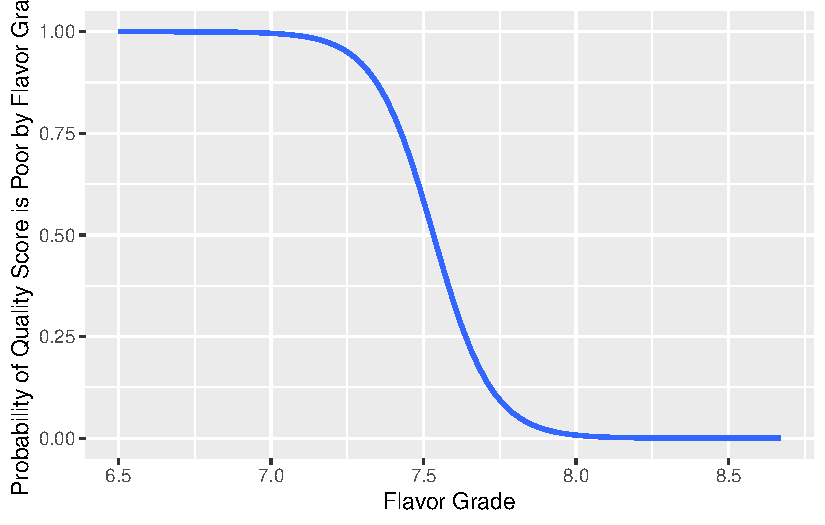
\includegraphics{project2draft_files/figure-pdf/fig-prob2-1.pdf}

}

\caption{\label{fig-prob2}Probability of Quality Score is Poor by Flavor
Grade.}

\end{figure}%

\begin{Shaded}
\begin{Highlighting}[]
\FunctionTok{ggplot}\NormalTok{(}\AttributeTok{data =}\NormalTok{ coffee1, }\FunctionTok{aes}\NormalTok{(}\AttributeTok{x =}\NormalTok{ acidity, }\AttributeTok{y =}\NormalTok{ probs.poor)) }\SpecialCharTok{+}
  \FunctionTok{geom\_smooth}\NormalTok{(}\AttributeTok{method=}\StringTok{"glm"}\NormalTok{, }
              \AttributeTok{method.args =} \FunctionTok{list}\NormalTok{(}\AttributeTok{family=}\StringTok{"binomial"}\NormalTok{), }
              \AttributeTok{se =} \ConstantTok{FALSE}\NormalTok{) }\SpecialCharTok{+}
  \FunctionTok{labs}\NormalTok{(}\AttributeTok{x =} \StringTok{"Acidity Grade"}\NormalTok{, }
       \AttributeTok{y =} \StringTok{"Probability of Quality Score is Poor by Acidity Grade"}\NormalTok{)}
\end{Highlighting}
\end{Shaded}

\begin{figure}[H]

\centering{

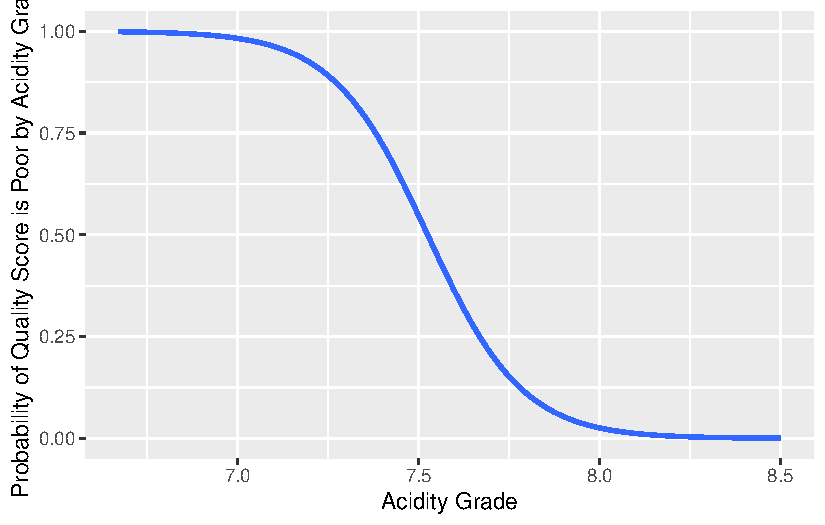
\includegraphics{project2draft_files/figure-pdf/fig-prob3-1.pdf}

}

\caption{\label{fig-prob3}Probability of Quality Score is Poor by
Acidity Grade.}

\end{figure}%

\begin{Shaded}
\begin{Highlighting}[]
\FunctionTok{ggplot}\NormalTok{(}\AttributeTok{data =}\NormalTok{ coffee1, }\FunctionTok{aes}\NormalTok{(}\AttributeTok{x =}\NormalTok{ altitude\_mean\_meters, }\AttributeTok{y =}\NormalTok{ probs.poor)) }\SpecialCharTok{+}
  \FunctionTok{geom\_smooth}\NormalTok{(}\AttributeTok{method=}\StringTok{"glm"}\NormalTok{, }
              \AttributeTok{method.args =} \FunctionTok{list}\NormalTok{(}\AttributeTok{family=}\StringTok{"binomial"}\NormalTok{), }
              \AttributeTok{se =} \ConstantTok{FALSE}\NormalTok{) }\SpecialCharTok{+}
  \FunctionTok{labs}\NormalTok{(}\AttributeTok{x =} \StringTok{"altitude\_mean\_meters Grade"}\NormalTok{, }
       \AttributeTok{y =} \StringTok{"Probability of Quality Score is Poor by altitude\_mean\_meters Grade"}\NormalTok{)}
\end{Highlighting}
\end{Shaded}

\begin{figure}[H]

\centering{

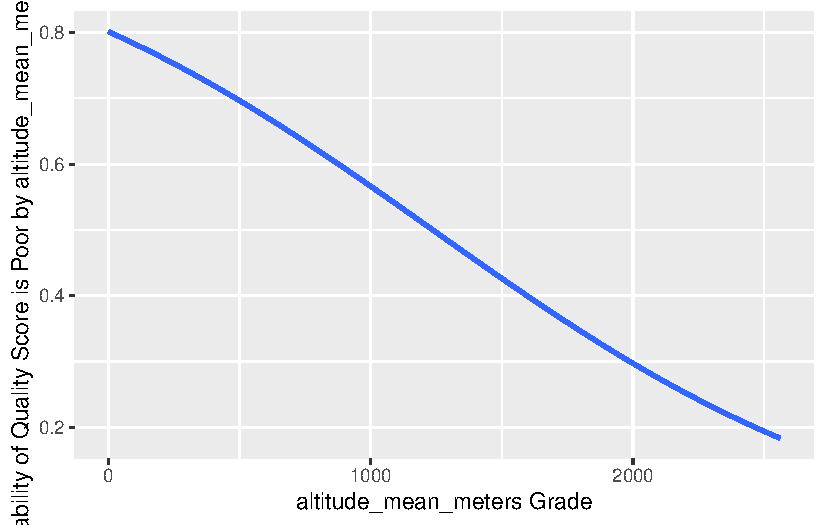
\includegraphics{project2draft_files/figure-pdf/fig-prob4-1.pdf}

}

\caption{\label{fig-prob4}Probability of Quality Score is Poor by
altitude\_mean\_meters Grade.}

\end{figure}%

\begin{Shaded}
\begin{Highlighting}[]
\FunctionTok{ggplot}\NormalTok{(}\AttributeTok{data =}\NormalTok{ coffee1, }\FunctionTok{aes}\NormalTok{(}\AttributeTok{x =}\NormalTok{ acidity, }\AttributeTok{y =}\NormalTok{ probs.poor)) }\SpecialCharTok{+}
  \FunctionTok{geom\_smooth}\NormalTok{(}\AttributeTok{method=}\StringTok{"glm"}\NormalTok{, }
              \AttributeTok{method.args =} \FunctionTok{list}\NormalTok{(}\AttributeTok{family=}\StringTok{"binomial"}\NormalTok{), }
              \AttributeTok{se =} \ConstantTok{FALSE}\NormalTok{) }\SpecialCharTok{+}
  \FunctionTok{labs}\NormalTok{(}\AttributeTok{x =} \StringTok{"Harvested Grade"}\NormalTok{, }
       \AttributeTok{y =} \StringTok{"Probability of Quality Score is Poor by Harvested Grade"}\NormalTok{)}
\end{Highlighting}
\end{Shaded}

\begin{figure}[H]

\centering{

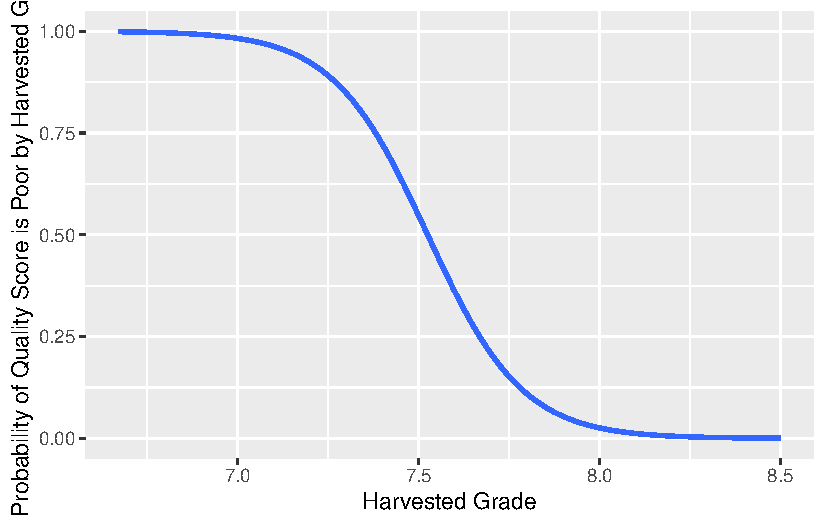
\includegraphics{project2draft_files/figure-pdf/fig-prob5-1.pdf}

}

\caption{\label{fig-prob5}Probability of Quality Score is Poor by
Harvested Grade.}

\end{figure}%

As Figure~\ref{fig-prob1} shows the probability of the quality score
being classified as poor by aroma grade, the less the aroma grade , the
higher probability being classified as poor quality. It's reasonable to
have such shape as the median aroma grade is round 7.2 (recalled from
the Figure~\ref{fig-boxplot1} ) so the outliers (aroma grade equals to
zero) will be directly classified as poor quality with the probability
of 1.

Similar interpretations will used for Figure~\ref{fig-prob2},
Figure~\ref{fig-prob3} and Figure~\ref{fig-prob5}. These three plots
indicate the probabilities of the quality score being classified as poor
by flavor, acidity grade and harvested year. Again, the higher score of
the flavor grade, acidity grade or harvested year, the less probability
being classified as poor quality. According to
Figure~\ref{fig-boxplot3}, Figure~\ref{fig-boxplot4} and
Figure~\ref{fig-boxplot6}, it's also reasonable to have such shape: the
outliers (flavor grade equals to zero or acidity grade equals to zero)
and harvested year contains extreme low-altitude values (close to zero)
will be directly classified as poor quality with the probability of 1.

As Figure~\ref{fig-prob4} shows the probability of the quality score
being classified as poor by aroma grade, lower altitudes correspond to a
higher probability of being classified as poor quality, aligning with
Figure~\ref{fig-boxplot5}, where Poor quality coffee has more
low-altitude samples. The probability curve gradually declines,
indicating better quality at higher altitudes. It is also reasonable to
have such shape: the outliers (large number of altitude close to zero)
will be classified as poor quality with the probability of 0.8.

\section{Conclusion}\label{conclusion}

Sensory Attributes (Aroma, Flavor, Acidity) Are the Strongest
Predictors: Figures Figure~\ref{fig-prob1}, Figure~\ref{fig-prob2}, and
Figure~\ref{fig-prob3} confirm that higher aroma, flavor, and acidity
scores significantly reduce the probability of being classified as Poor
quality. Flavor has the largest impact, followed by aroma and acidity.
Boxplots (Figure~\ref{fig-boxplot1}, Figure~\ref{fig-boxplot2},
Figure~\ref{fig-boxplot3}) further show that Good quality coffee has
consistently higher sensory scores. Implication: Farmers should
prioritize improving flavor, aroma, and acidity through better
cultivation, harvesting, and processing techniques.

Altitude Has a Moderate but Significant Effect: Figure~\ref{fig-prob4}
shows that higher altitude correlates with better coffee quality, with
low-altitude coffee more likely to be classified as Poor.
Figure~\ref{fig-boxplot5} confirms that Good coffee tends to be grown at
higher altitudes, though outliers exist. Implication: Farmers in
higher-altitude regions may naturally produce higher-quality coffee,
while low-altitude farmers may need to focus on post-harvest processing
to compensate.

Harvested Year Has Limited Impact: Figure~\ref{fig-prob5} shows that
coffee from older harvests has a higher probability of being Poor,
aligning with Figure~\ref{fig-boxplot6}, where Poor quality coffee tends
to have older harvest years. However, the overlapping boxplots indicate
that harvest year alone does not strictly determine quality---some older
beans still maintain high quality. Implication: Farmers should focus on
proper storage and post-harvest processing to preserve quality over
time.

By implementing following improvements, local coffee farmers can enhance
their coffee quality and increase the chances of classification as
high-quality (Good) coffee. 1. Focus on enhancing sensory attributes
(Flavor, Aroma, Acidity) -- This has the greatest impact on quality
classification. 2. If growing at low altitudes, compensate with better
processing techniques -- Higher altitudes naturally favor quality, but
post-harvest handling can improve lower-altitude coffee. 3. Ensure
proper storage and handling of harvested beans -- Even older harvests
can maintain high quality if well-preserved. 4. Processing quality
matters more than defects or origin -- Farmers should focus on
fermentation, drying, and sorting techniques to maximize quality.




\end{document}
